\documentclass[11pt,a4paper]{ctexart} % 使用中文主流学术文档类，支持中文排版
\usepackage[utf8]{inputenc}
\usepackage{amsmath}   % 增强数学公式宏包
\usepackage{amssymb}   % 数学符号宏包
\usepackage{booktabs}  % 绘制学术论文标准三线表
\usepackage{graphicx}  % 插入图形宏包
\usepackage{float}     % 固定图表位置宏包 [H]
\usepackage{geometry}  % 调整页边距
\usepackage{hyperref}  % 超链接与PDF交叉引用
\usepackage{caption}   % 调整图表题干与字体
\usepackage{threeparttable} % 规范表格的脚注
\usepackage{siunitx}   % 规范科学计数法与单位排版
\usepackage{tabularx}  % 允许自动换行的自适应表格

% 设置页边距，满足标准学术论文要求
\geometry{left=2.5cm, right=2.5cm, top=3.0cm, bottom=3.0cm}

% 设置超链接颜色
\hypersetup{
    colorlinks=true,
    linkcolor=black,
    citecolor=black,
    urlcolor=black
}

% 设置图表标题字体大小与加粗
\captionsetup[table]{font=small, labelfont=bf, labelsep=quad}
\captionsetup[figure]{font=small, labelfont=bf, labelsep=quad}
\pagestyle{plain}

\title{\bfseries 基于机器学习分类算法的心力衰竭患者生存预后预测与临床风险因子识别研究}
\date{}

\begin{document}

\maketitle

\begin{abstract}
{\bfseries 背景与目的：} 心力衰竭（Heart Failure, HF）作为各种心血管疾病的终末期表现，具有极高的致死率与复杂的病理机理。准确评估患者的随访生存预后并识别核心临床高危因子，对优化分层诊疗及医疗资源调配具有重大临床价值。本研究旨在基于临床基线与实验室随访数据，构建高精度的生存预后分类预测模型，并量化对比传统机器学习、集成算法与全连接深度网络在医疗表格数据任务中的行为差异与过拟合风险。
{\bfseries 方法：} 本研究基于 299 例心力衰竭患者的连续随访临床数据集。首先对严重右偏分布的血清肌酐与肌酸激酶实施对数变换 $\log(1+x)$ 平滑清洗，运用卡方检验与 Wilcoxon 秩和检验的双轨统计学方法验证特征组间显著性差异。随后，构建了逻辑回归（LR）、随机森林（RF）、极端梯度提升树（XGBoost）以及多层感知机深度学习网络（MLP）四种分类模型，在 8:2 的分层抽样独立测试集上进行泛化性能的横向横评，引入 AUC 泛化衰减率定量评估结构过拟合。
{\bfseries 结果：} 统计检验与机器学习特征重要性排序高度契合，共同锁定随访时间、射血分数与血清肌酐为三大核心驱动因子（$p < 0.0001$）。在独立测试集表现中，传统机器学习与集成算法展现出高度稳健的分类准确率（\num{81.67}\%），其中随机森林（RF）凭借最高的曲线下面积（$\text{AUC} = 0.88$）和最优的 F1-Score（\num{0.6857}）综合表现最佳，其临床漏诊率显著低于其他对比模型。全连接深度学习模型（MLP）在缺乏空间与时间先验的医疗表格数据中表现出严重的过拟合倾向（训练集 $\text{AUC} = 1.0000$），导致其测试集准确率骤降至 \num{70.00}\%，$\text{AUC}$ 泛化衰减率高达 \num{0.2323}。
{\bfseries 结论：} 传统机器学习与集成算法在应对小样本医疗表格数据时，具有显著优于无先验深度学习网络的泛化鲁棒性与抗噪性能；提取的临床风险因子具备高度的病理学可解释性，能为心衰临床决策支持系统（CDSS）的高效风险分层提供可靠的数学依据。
\end{abstract}

\noindent\hangindent=1.5em\textbf{关键词：} 心力衰竭；机器学习；生存预测；特征选择；过拟合；深度学习

\newpage

\section{引言}
心力衰竭（Heart Failure, HF）是各类心血管疾病进展至终末期的复杂临床综合征，其本质为心脏泵血功能受损，心输出量无法满足机体组织代谢需求，进而引发多器官功能障碍，具有高住院率、高再入院率及高远期病死率的显著特征\cite{chicco2020machine}。全球范围内，心力衰竭的疾病负担持续加重，患病人数从1990年的3350万快速增长至2017年的6430万，已成为公共卫生领域面临的重大挑战之一\cite{newaz2021survival}。我国心力衰竭人群基数庞大，随着人口老龄化加剧及慢性病患病率上升，其发病率、致残率与病死率长期居高不下，不仅严重影响患者生存质量，也给临床诊疗体系与社会医疗资源带来沉重负担\cite{benjamin2019heart}。

精准的生存预后评估与个体化风险分层是心力衰竭临床诊疗的关键环节，对制定合理治疗策略、优化医疗资源配置、改善患者远期结局具有不可替代的指导价值\cite{ponikowski2014heart}。准确识别高死亡风险患者并预判其疾病进展轨迹，有助于临床医师及时采取强化干预措施；而有效甄别低危人群，则可避免不必要的过度检查与过度治疗，减轻患者心理压力与经济负担。然而，心力衰竭的病理生理机制极为复杂，其发生发展受年龄、心功能状态、肾功能水平、电解质紊乱及多种合并症等多维度临床指标的共同影响，传统单指标分层方法或常规风险评分系统难以有效捕捉变量间的非线性高阶交互关系，导致临床预后评估的准确性、时效性与稳定性均存在明显局限\cite{ahmad2022survival}。

近年来，电子健康档案（Electronic Health Records, EHR）的广泛普及与医学数据科学的快速发展，为心力衰竭预后预测提供了新的技术路径与研究思路\cite{shickel2018deep}。机器学习技术能够从海量、高维、异构的临床数据中自动挖掘潜在关联与隐性规律，构建数据驱动的精准预测模型，弥补传统统计方法在非线性拟合与复杂关联捕捉上的不足，为临床决策支持系统（Clinical Decision Support System, CDSS）的研发奠定了坚实基础。然而，医疗临床表格数据普遍存在样本量有限、连续变量呈非正态右偏分布、特征间存在多重共线性、类别分布不平衡等固有问题，这些特性对模型的泛化能力、抗噪声干扰能力及临床可解释性提出了更高要求，也使得不同算法在医疗小样本任务中的表现差异显著\cite{tabular2022}。

为此，本研究旨在构建兼顾预测精度、泛化鲁棒性与临床可解释性的心力衰竭患者生存预后预测模型，并系统识别影响其远期生存结局的核心临床风险因子。基于公开心力衰竭临床随访数据集，本研究首先对偏态分布特征实施对数变换预处理，再构建逻辑回归、随机森林、极端梯度提升树与多层感知机四种不同机理的预测模型，在分层抽样的独立测试集上横向对比其泛化性能，并引入AUC泛化衰减率定量评估模型的过拟合风险，最终明确适用于小样本医疗表格数据的最优建模策略。研究结果不仅可为心力衰竭患者的个体化风险分层提供客观、可靠的量化依据，也能为心血管疾病领域临床决策支持系统的开发与临床干预方案的优化提供科学参考。研究整体的研究技术路线如图 \ref{fig:workflow} 所示。

\begin{figure}[H]
    \centering
    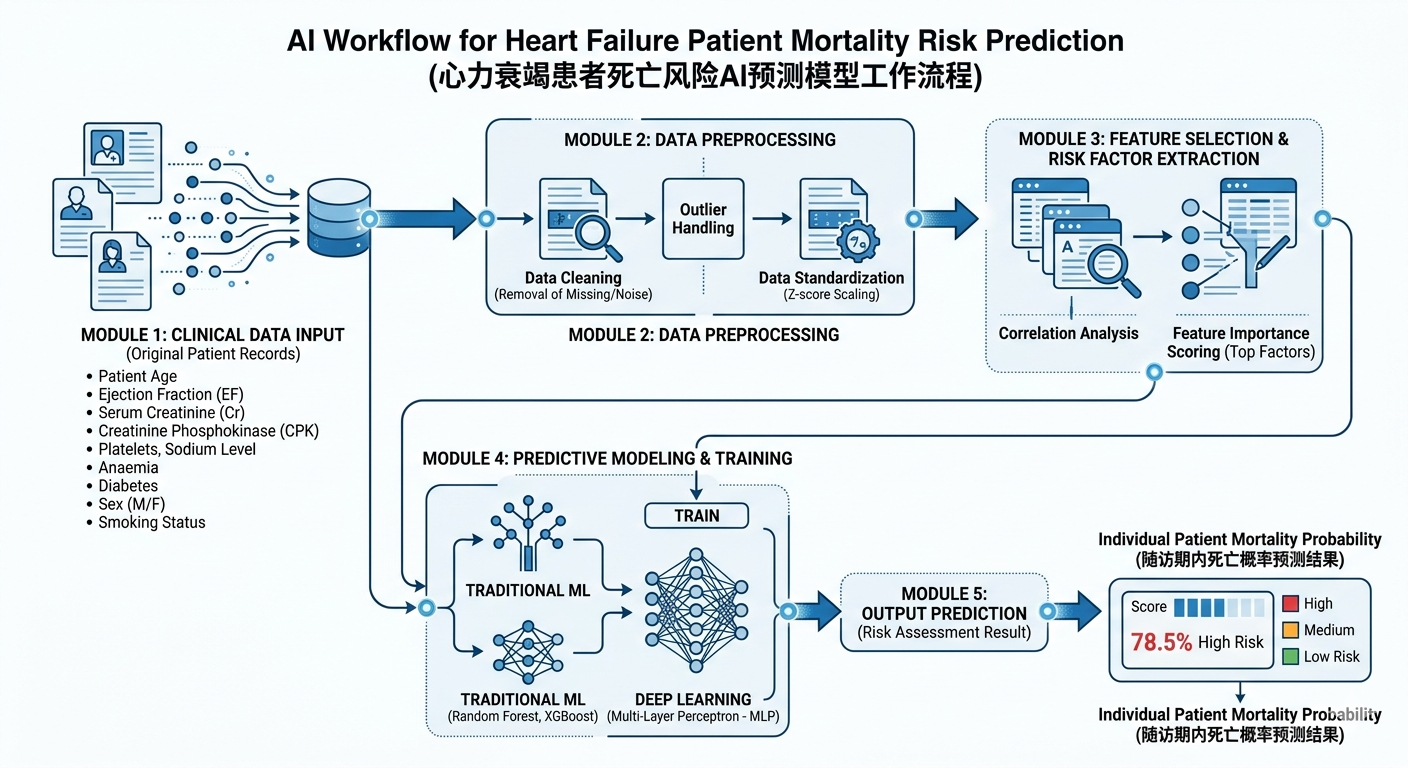
\includegraphics[width=0.85\textwidth]{workflow.png}
    \caption{基于机器学习与深度学习的心力衰竭患者生存预后预测流线图}
    \label{fig:workflow}
    \vspace{-10pt}
\end{figure}

\section{材料与方法}

\subsection{数据集来源与基线特征}
本研究采用公开心力衰竭临床随访数据集开展回顾性研究。该数据集为公开共享的临床研究数据集，数据结构规范、临床指标完整，具有良好的研究适用性。数据集共包含299例心力衰竭确诊患者的连续随访记录，涵盖7项连续变量、5项二分类变量及1项生存结局标签，结局标签中0代表随访期内生存、1代表随访期内死亡。数据集无缺失值、无明显异常标记，数据质量可靠，可直接用于统计分析与模型构建。样本结局分布中，生存患者203例、死亡患者96例，死亡事件占比约32.11\%，呈现轻度类别不平衡，符合临床随访数据的一般特征。

\subsection{数据预处理与偏态平滑}
在数据探索性分析阶段发现，血清肌酐与肌酸激酶两项实验室指标呈现明显右偏分布，存在大量极端高值。这类偏态数据易造成线性模型权重偏倚、降低梯度类算法收敛效率，因此需要进行合理校正。为此，本研究采用$\log(1+x)$对数变换对两项偏态指标进行平滑处理。该变换在保留变量单调性的同时压缩极端值影响，并避免$\log(x)$在零值处无定义的问题。本研究不直接剔除异常值，而是通过变换降低极端值干扰，最大限度保留样本信息。

此外，为消除不同特征量纲差异对模型训练的影响，逻辑回归与多层感知机对输入特征敏感，因此在模型输入前对所有连续变量执行Z‑score标准化，使其服从均值为0、方差为1的标准正态分布；树模型（随机森林、XGBoost）不受量纲影响，无需标准化。

\subsection{临床特征分析与双轨统计学检验}
为确保特征筛选的科学性与临床可解释性，本研究采用统计学检验与机器学习特征重要性相结合的双轨验证策略。首先采用Shapiro‑Wilk正态性检验，结果显示多数连续变量不满足正态分布，因此选用非参数Wilcoxon秩和检验比较存活组与死亡组的分布差异；二分类特征则采用Pearson卡方检验，分析其与生存结局的关联性。

统计学检验属于过滤式筛选，侧重单变量显著性；而随机森林特征重要性属于封装式筛选，可捕捉变量间非线性交互效应。两种方法相互印证、互为补充，可有效减少单一筛选带来的偏倚，提高特征选择的可靠性与临床可解释性。

\subsection{机器学习与深度学习模型配置}
为系统比较不同算法在小样本医疗表格数据中的表现，本研究选取覆盖线性模型、集成树模型、梯度提升模型及深度网络的四类代表性算法，全面评估模型的拟合能力、抗噪性与泛化稳定性。

实验采用分层随机抽样，按照8:2比例划分训练集（$N=239$）与独立测试集（$N=60$），确保两组数据的死亡事件比例与总体一致，避免因类别分布差异引入模型偏差。模型超参考心衰机器学习研究的常用经验值，并在小范围内进行验证优化，以保证模型稳定可靠。

逻辑回归作为传统线性基准模型，其核心概率映射通过$Sigmoid$函数实现：
\begin{equation}
    \sigma(z) = \frac{1}{1+e^{-z}}
\end{equation}

本研究构建的模型架构与超参数配置如下：
\begin{itemize}
    \item \textbf{逻辑回归（LR）：} 采用$L_2$正则化惩罚项以规避共线性，最大迭代次数为1000次；
    \item \textbf{随机森林（RF）：} 包含100棵决策树的集成森林，不限制树深，以基尼不纯度作为分裂标准；
    \item \textbf{XGBoost（XGB）：} 以树模型为基分类器，迭代次数设为100，学习率$\eta=0.1$，采用对数损失函数执行残差迭代；
    \item \textbf{多层感知机（MLP）：} 构建了一个包含3个全连接层的深度神经网络，结构为“输入$\to$32神经元$\to$ReLU$\to$Dropout(0.2)$\to$16神经元$\to$ReLU$\to$输出$\to$Sigmoid”，使用Adam优化器，学习率设定为0.01，共训练50个Epoch。
\end{itemize}

\subsection{模型评估指标}
考虑到心衰数据存在类别不平衡问题，单一准确率易高估模型性能、无法反映高危患者识别能力，因此本研究采用多维度综合评估体系。模型泛化性能评估采用独立测试集上的准确率、精确率、召回率、F1值，计算公式如下：
\begin{equation}
    F_1 = 2 \cdot \frac{\text{Precision} \cdot \text{Recall}}{\text{Precision} + \text{Recall}}
\end{equation}

其中，召回率重点反映高危患者检出能力，具有明确临床价值；精确率体现预测阳性结果的可靠性；F1‑Score平衡两者表现。同时利用受试者工作特征曲线下面积（ROC‑AUC）综合评估模型整体区分能力，该指标不受类别分布影响。

为进一步量化模型泛化能力，定义AUC泛化衰减率：$\text{Drop} = \text{AUC}_{\text{Train}} - \text{AUC}_{\text{Test}}$，直接反映模型过拟合程度；同时结合混淆矩阵直观呈现真阳性、假阳性、真阴性、假阴性分布，便于临床结果解释。

\subsection{模型评估指标}
为全面评估模型在不平衡数据下的分类性能，本研究采用独立测试集上的多项量化指标，包括准确率（Accuracy）、精确率（Precision）、召回率（Recall）及F1值（F1‑Score），其中F1值计算公式如下：
\begin{equation}
    F_1 = 2 \cdot \frac{\text{Precision} \cdot \text{Recall}}{\text{Precision} + \text{Recall}}
\end{equation}

同时，采用受试者工作特征曲线下面积（ROC‑AUC）综合评估模型的整体分类能力。为量化模型过拟合程度，定义AUC泛化衰减率（Drop）：$\text{Drop} = \text{AUC}_{\text{Train}} - \text{AUC}_{\text{Test}}$，用于衡量模型在训练集与测试集上的性能差异。

\section{结果与分析}

\subsection{临床特征基线统计与对数变换成效}
本研究首先对心力衰竭患者基线临床特征进行全面描述性统计，以明确总体分布、存活组与死亡组间的差异模式。研究队列共包含299例心衰患者，其中存活者203例（67.89\%）、死亡者96例（32.11\%），数据呈现轻度类别不平衡，符合真实临床随访数据的分布特征。基线统计结果显示，两组患者在年龄、射血分数、血清肌酐及随访时间方面存在显著差异；而贫血、糖尿病、高血压、性别、吸烟等指标在两组间分布相近，未表现出明显组间差异。上述结果提示，心功能、肾功能及年龄相关指标可能与心衰患者远期生存密切相关。详细基线统计结果如表 \ref{tab:baseline} 所示。

\begin{table}[H]
\centering
\caption{心力衰竭队列患者基线临床特征统计表}
\label{tab:baseline}
\small
\begin{tabular}{lrrr}
\toprule
\textbf{临床特征} & \textbf{总体人群 (N=29)} & \textbf{存活组 (n=203)} & \textbf{死亡组 (n=96)} \\
\midrule
\texttt{年龄} (岁) & $60.83 \pm 11.89$ & $58.76 \pm 10.64$ & $65.22 \pm 13.21$ \\
\texttt{贫血} (\%) & \num{43.14}\% & \num{40.89}\% & \num{47.92}\% \\
\texttt{肌酸磷酸激酶} (U/L) & $581.84 \pm 970.29$ & $540.05 \pm 753.80$ & $670.20 \pm 1316.58$ \\
\texttt{糖尿病} (\%) & \num{41.81}\% & \num{41.87}\% & \num{41.67}\% \\
\texttt{射血分数} (\%) & $38.08 \pm 11.83$ & $40.27 \pm 10.86$ & $33.47 \pm 12.53$ \\
\texttt{高血压} (\%) & \num{35.12}\% & \num{32.51}\% & \num{40.62}\% \\
\texttt{血小板计数} ($\times 10^3/\mu\text{L}$) & $263358.03 \pm 97804.24$ & $266657.49 \pm 97531.20$ & $256381.04 \pm 98525.68$ \\
\texttt{血清肌酐} (mg/dL) & $1.39 \pm 1.03$ & $1.18 \pm 0.65$ & $1.84 \pm 1.47$ \\
\texttt{血清钠} (mEq/L) & $136.63 \pm 4.41$ & $137.22 \pm 3.98$ & $135.38 \pm 5.00$ \\
\texttt{性别} (\%) & \num{64.88}\% & \num{65.02}\% & \num{64.58}\% \\
\texttt{吸烟} (\%) & \num{32.11}\% & \num{32.51}\% & \num{31.25}\% \\
\texttt{随访时间} (天) & $130.26 \pm 77.61$ & $158.34 \pm 67.74$ & $70.89 \pm 62.38$ \\
\bottomrule
\end{tabular}
\begin{tablenotes}
    \footnotesize
    \item 注：连续变量以均值$\pm$标准差表示；分类变量以百分比表示。
\end{tablenotes}
\end{table}

数据探索发现，血清肌酐与肌酸磷酸激酶两项实验室指标呈极端右偏分布，原始偏度分别为4.43、4.44，峰度高达24–25，存在大量异常高值，极易干扰线性模型权重估计与梯度收敛。为有效抑制极端值影响、改善分布对称性，本研究采用$\log(1+x)$对数变换进行偏态校正。变换后，肌酸磷酸激酶偏度降至0.42、峰度降至-0.34，血清肌酐偏度降至2.30、峰度降至7.07，分布形态显著改善，为后续建模提供更稳定的数据基础。对数变换前后偏度、峰度对比见表 \ref{tab:skewness}，分布变化见图 \ref{fig:creatinine_log}。

\begin{table}[H]
\centering
\caption{核心连续变量对数变换前后偏态与峰度对照表}
\label{tab:skewness}
\small
\begin{tabular}{lrrrr}
\toprule
\textbf{临床连续特征} & \textbf{变换前偏度} & \textbf{变换后偏度 } & \textbf{变换前峰度} & \textbf{变换后峰度} \\
\midrule
\texttt{血清肌酐} & $4.4336$ & $2.3016$ & $25.3783$ & $7.0721$ \\
\texttt{肌酸磷酸激酶} & $4.4407$ & $0.4206$ & $24.7105$ & $-0.3403$ \\
\bottomrule
\end{tabular}
\end{table}

\begin{figure}[H]
    \centering
    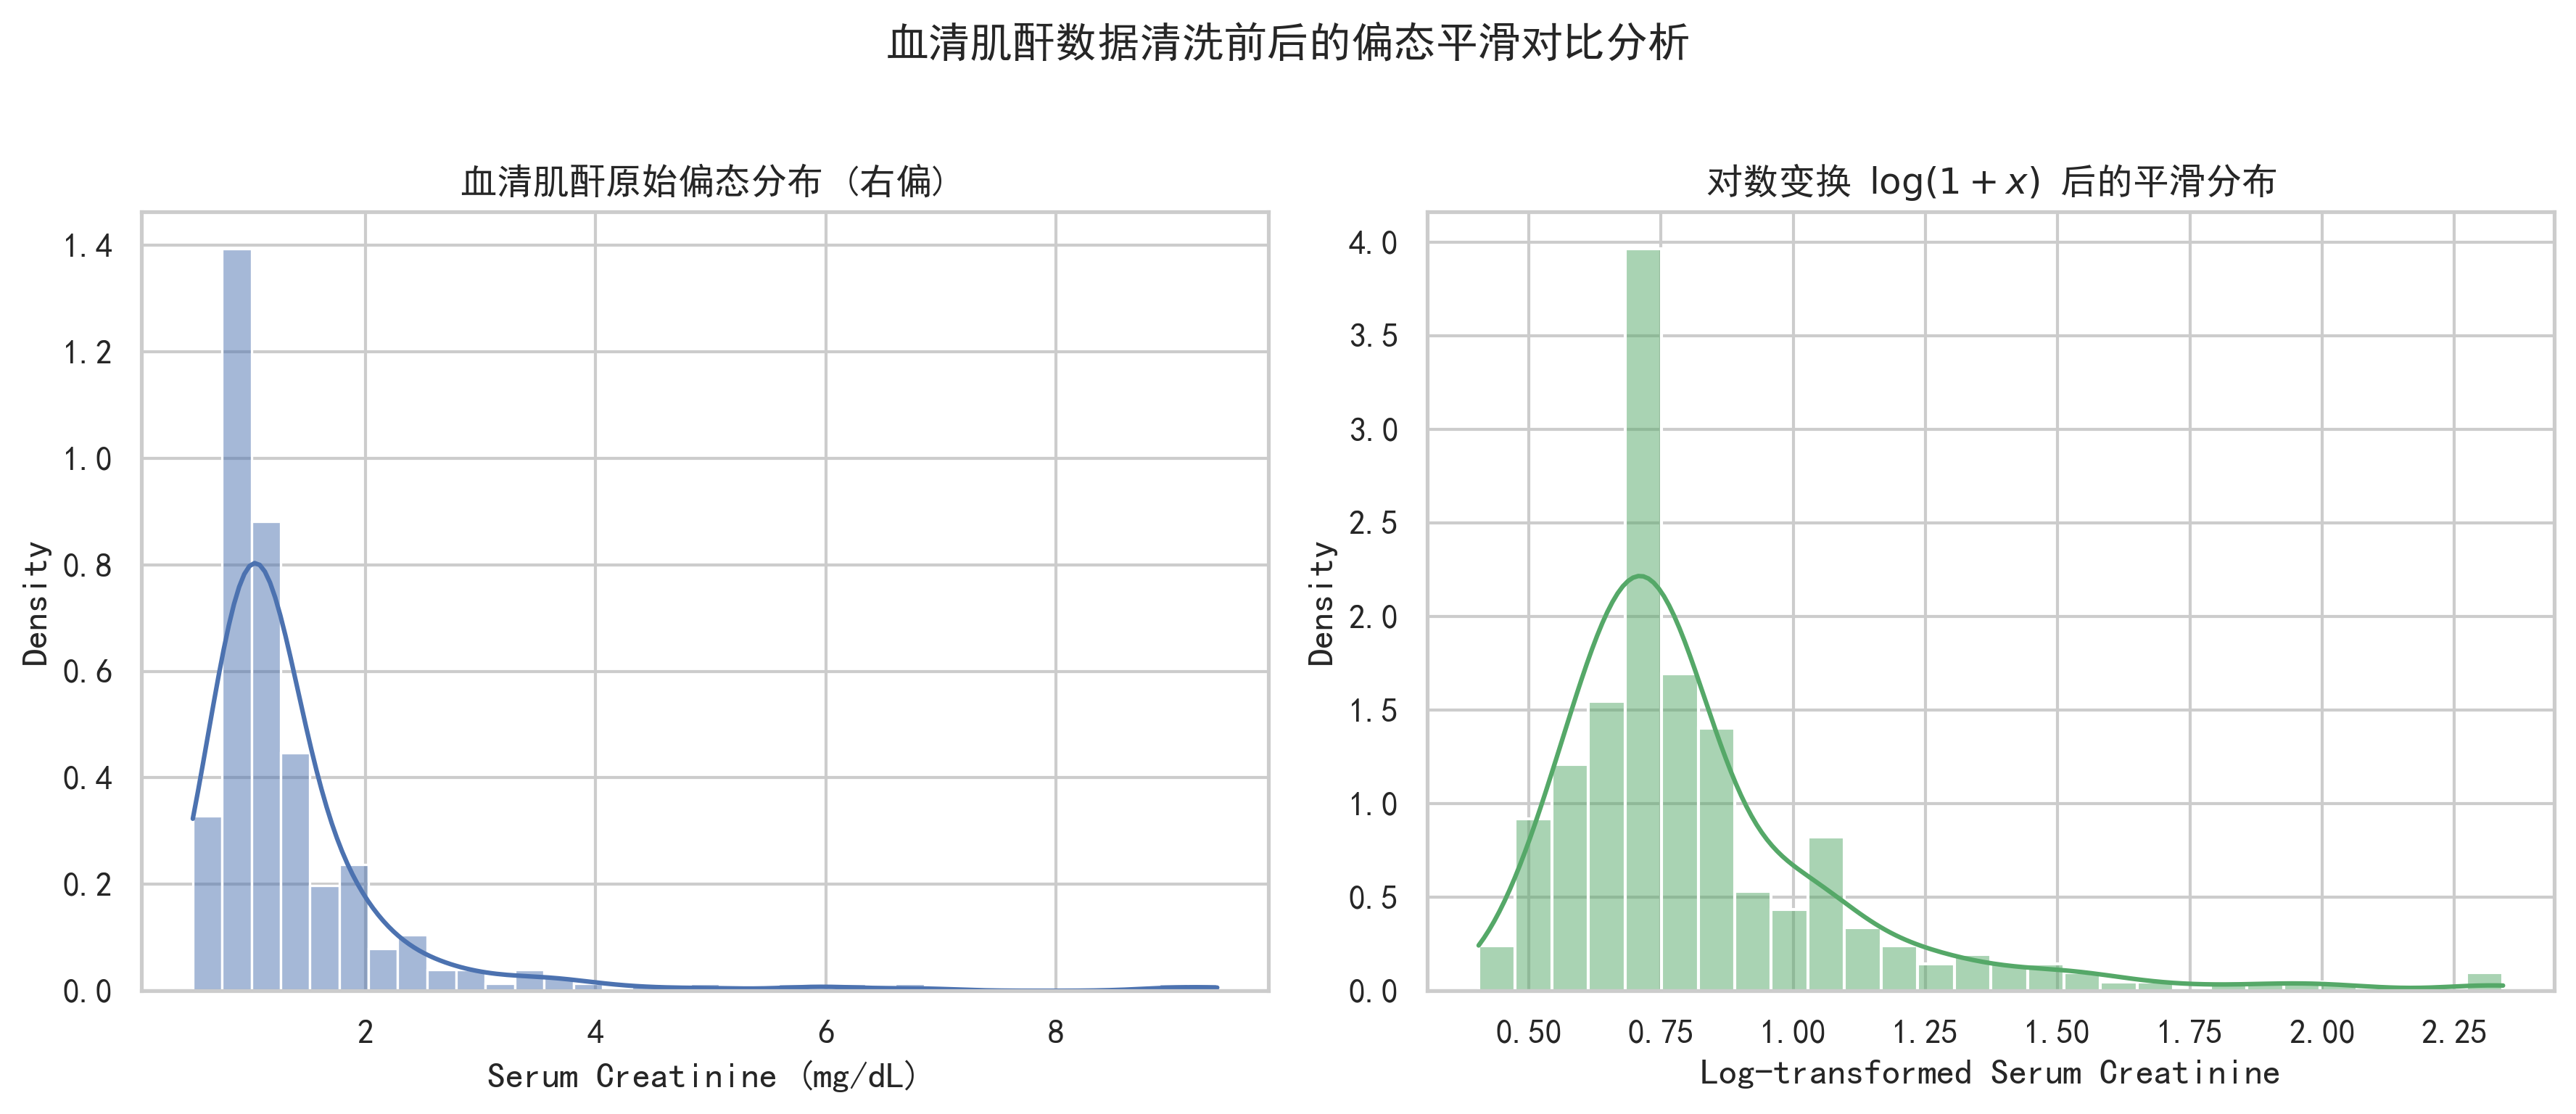
\includegraphics[width=0.75\textwidth]{血清肌酐对数变换前后分布对比图.png}
    \caption{血清肌酐与肌酸激酶对数变换前后分布偏态平滑对照图}
    \label{fig:creatinine_log}
\end{figure}

\subsection{特征相关性与风险因子显著性检验}
为科学筛选心衰预后关键预测因子，本研究采用统计学检验与机器学习特征重要性相结合的双轨验证策略。相关性分析显示，多数临床指标间相关性较弱，未出现严重多重共线性；随机森林特征重要性排序与组间检验结果高度吻合，共同揭示了心衰死亡风险的核心驱动因子。结果汇总于表 \ref{tab:importance}、图 \ref{fig:heatmap} 与图 \ref{fig:importance}。

\begin{figure}[H]
    \centering
    \begin{minipage}[t]{0.48\textwidth}
        \centering
        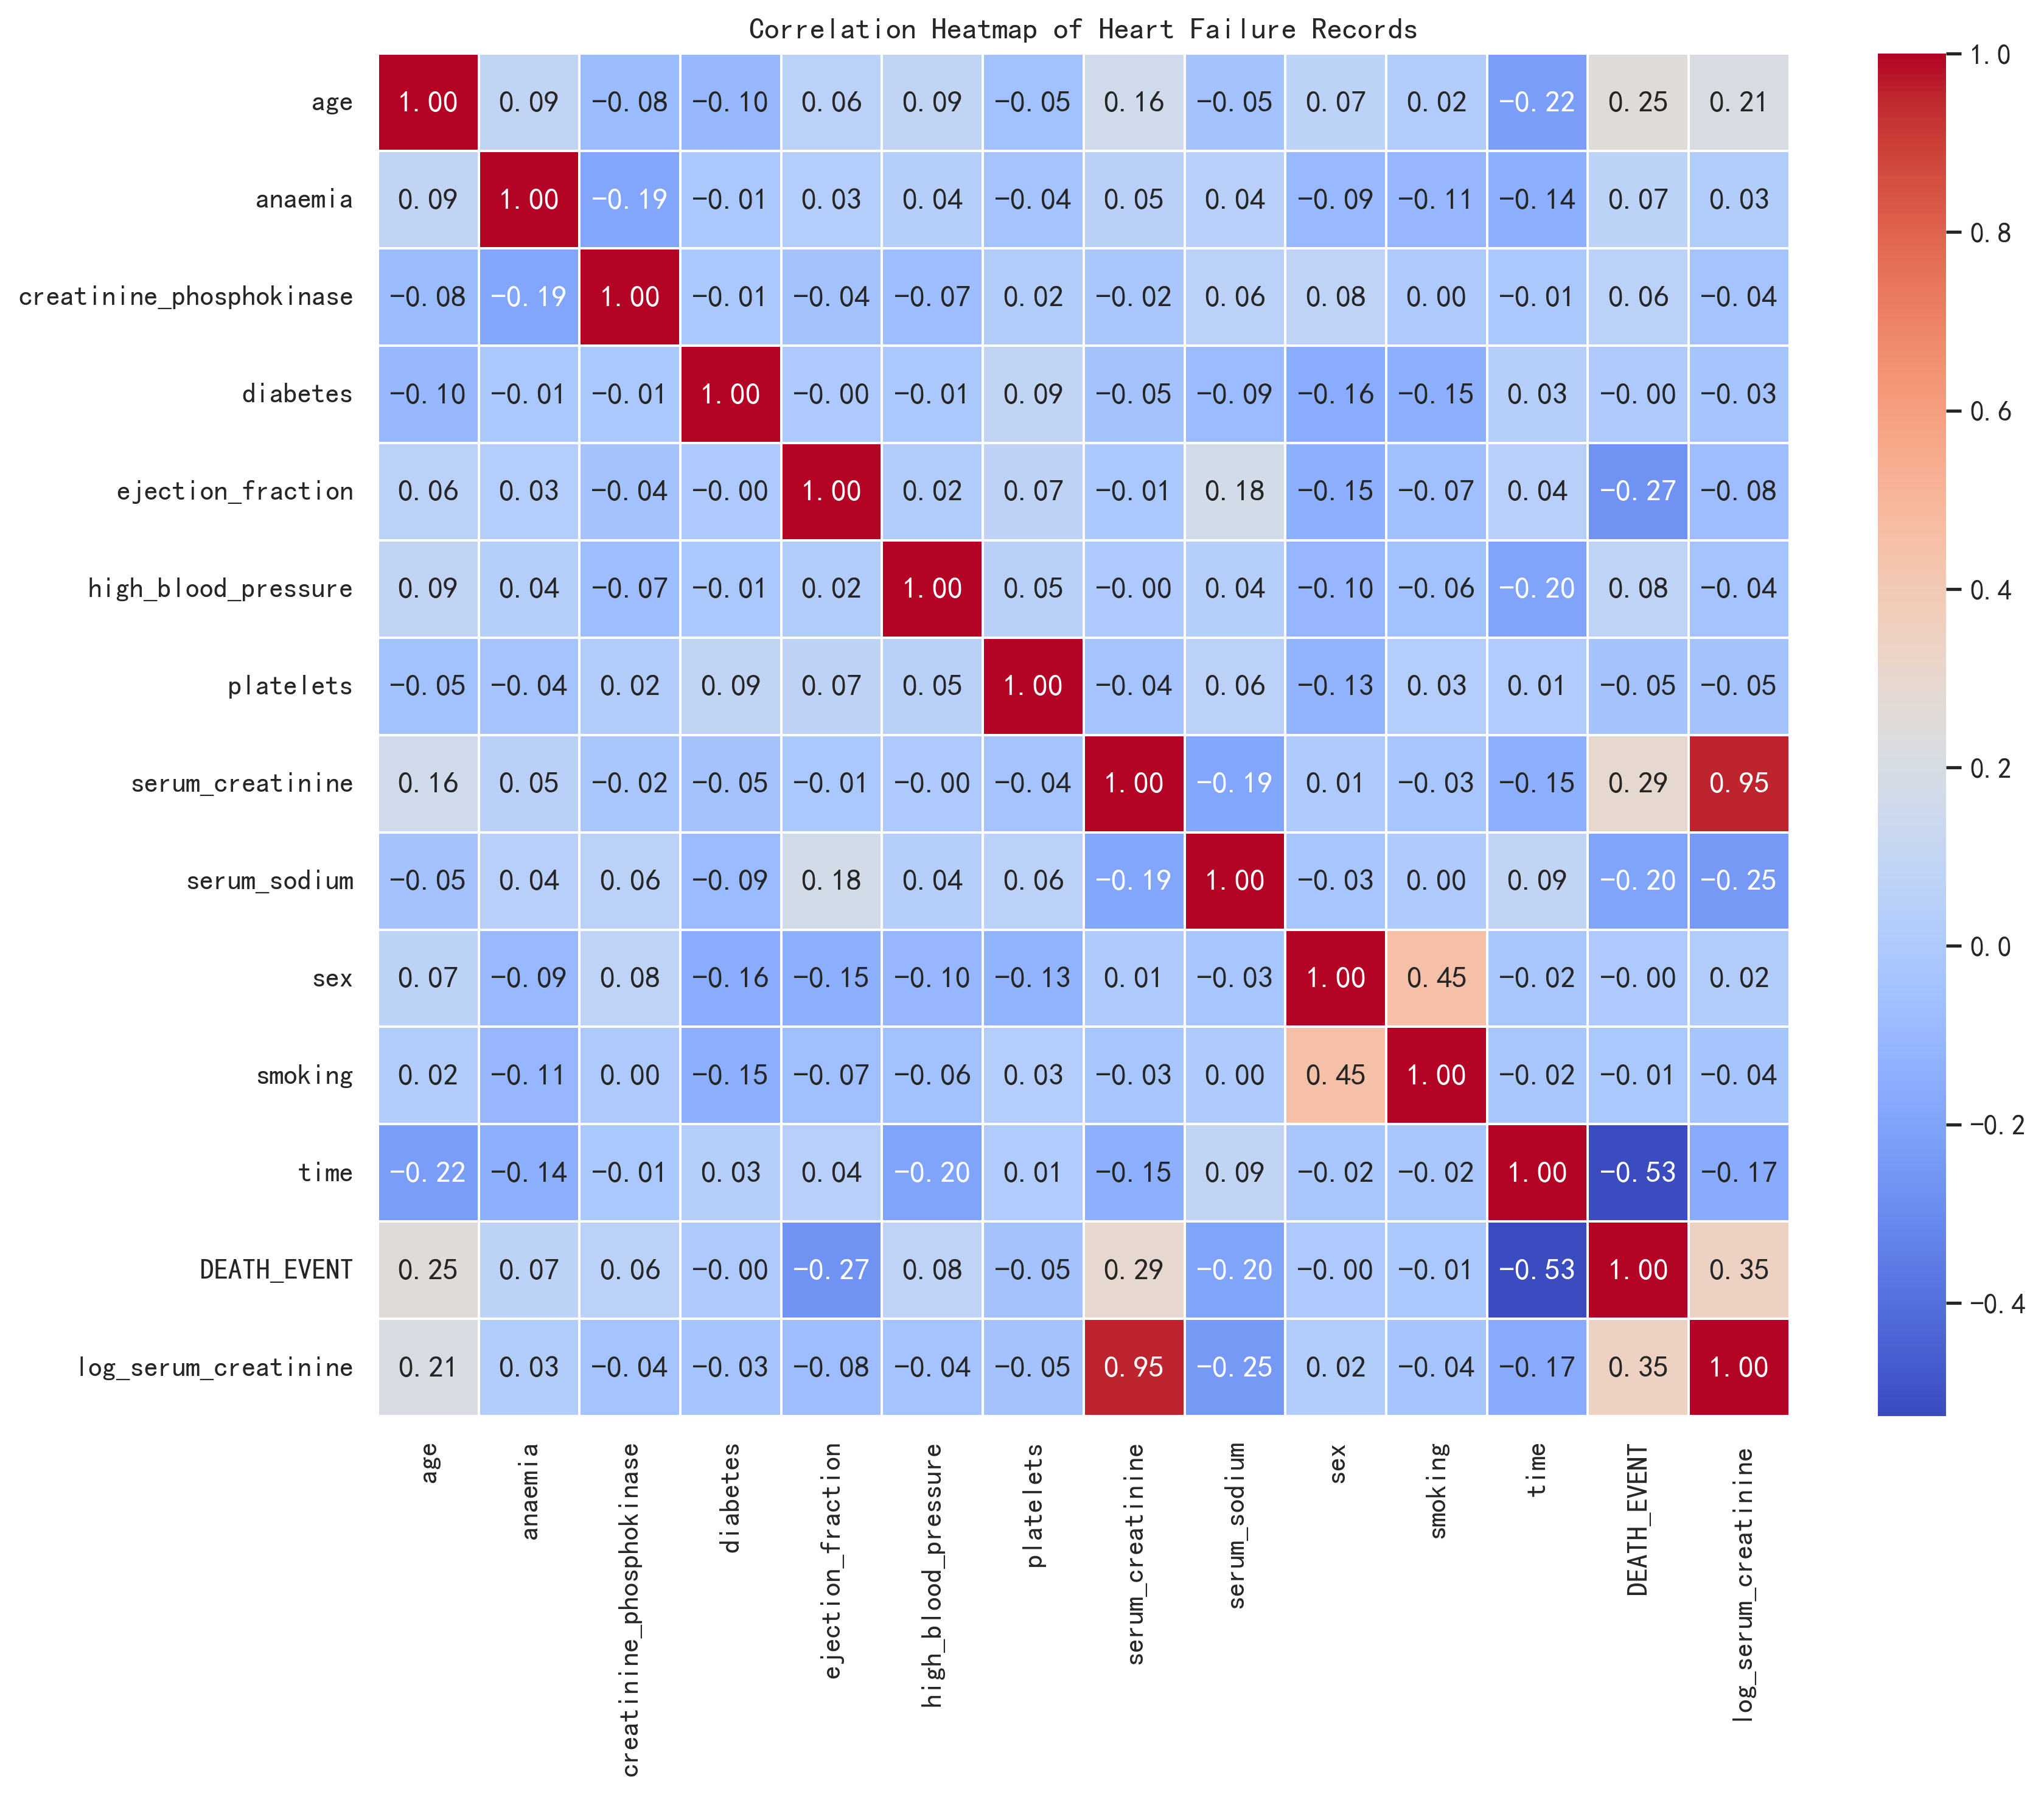
\includegraphics[width=\textwidth]{heatmap.png}
        \caption{临床特征特征间相关性热力图}
        \label{fig:heatmap}
    \end{minipage}
    \hfill
    \begin{minipage}[t]{0.48\textwidth}
        \centering
        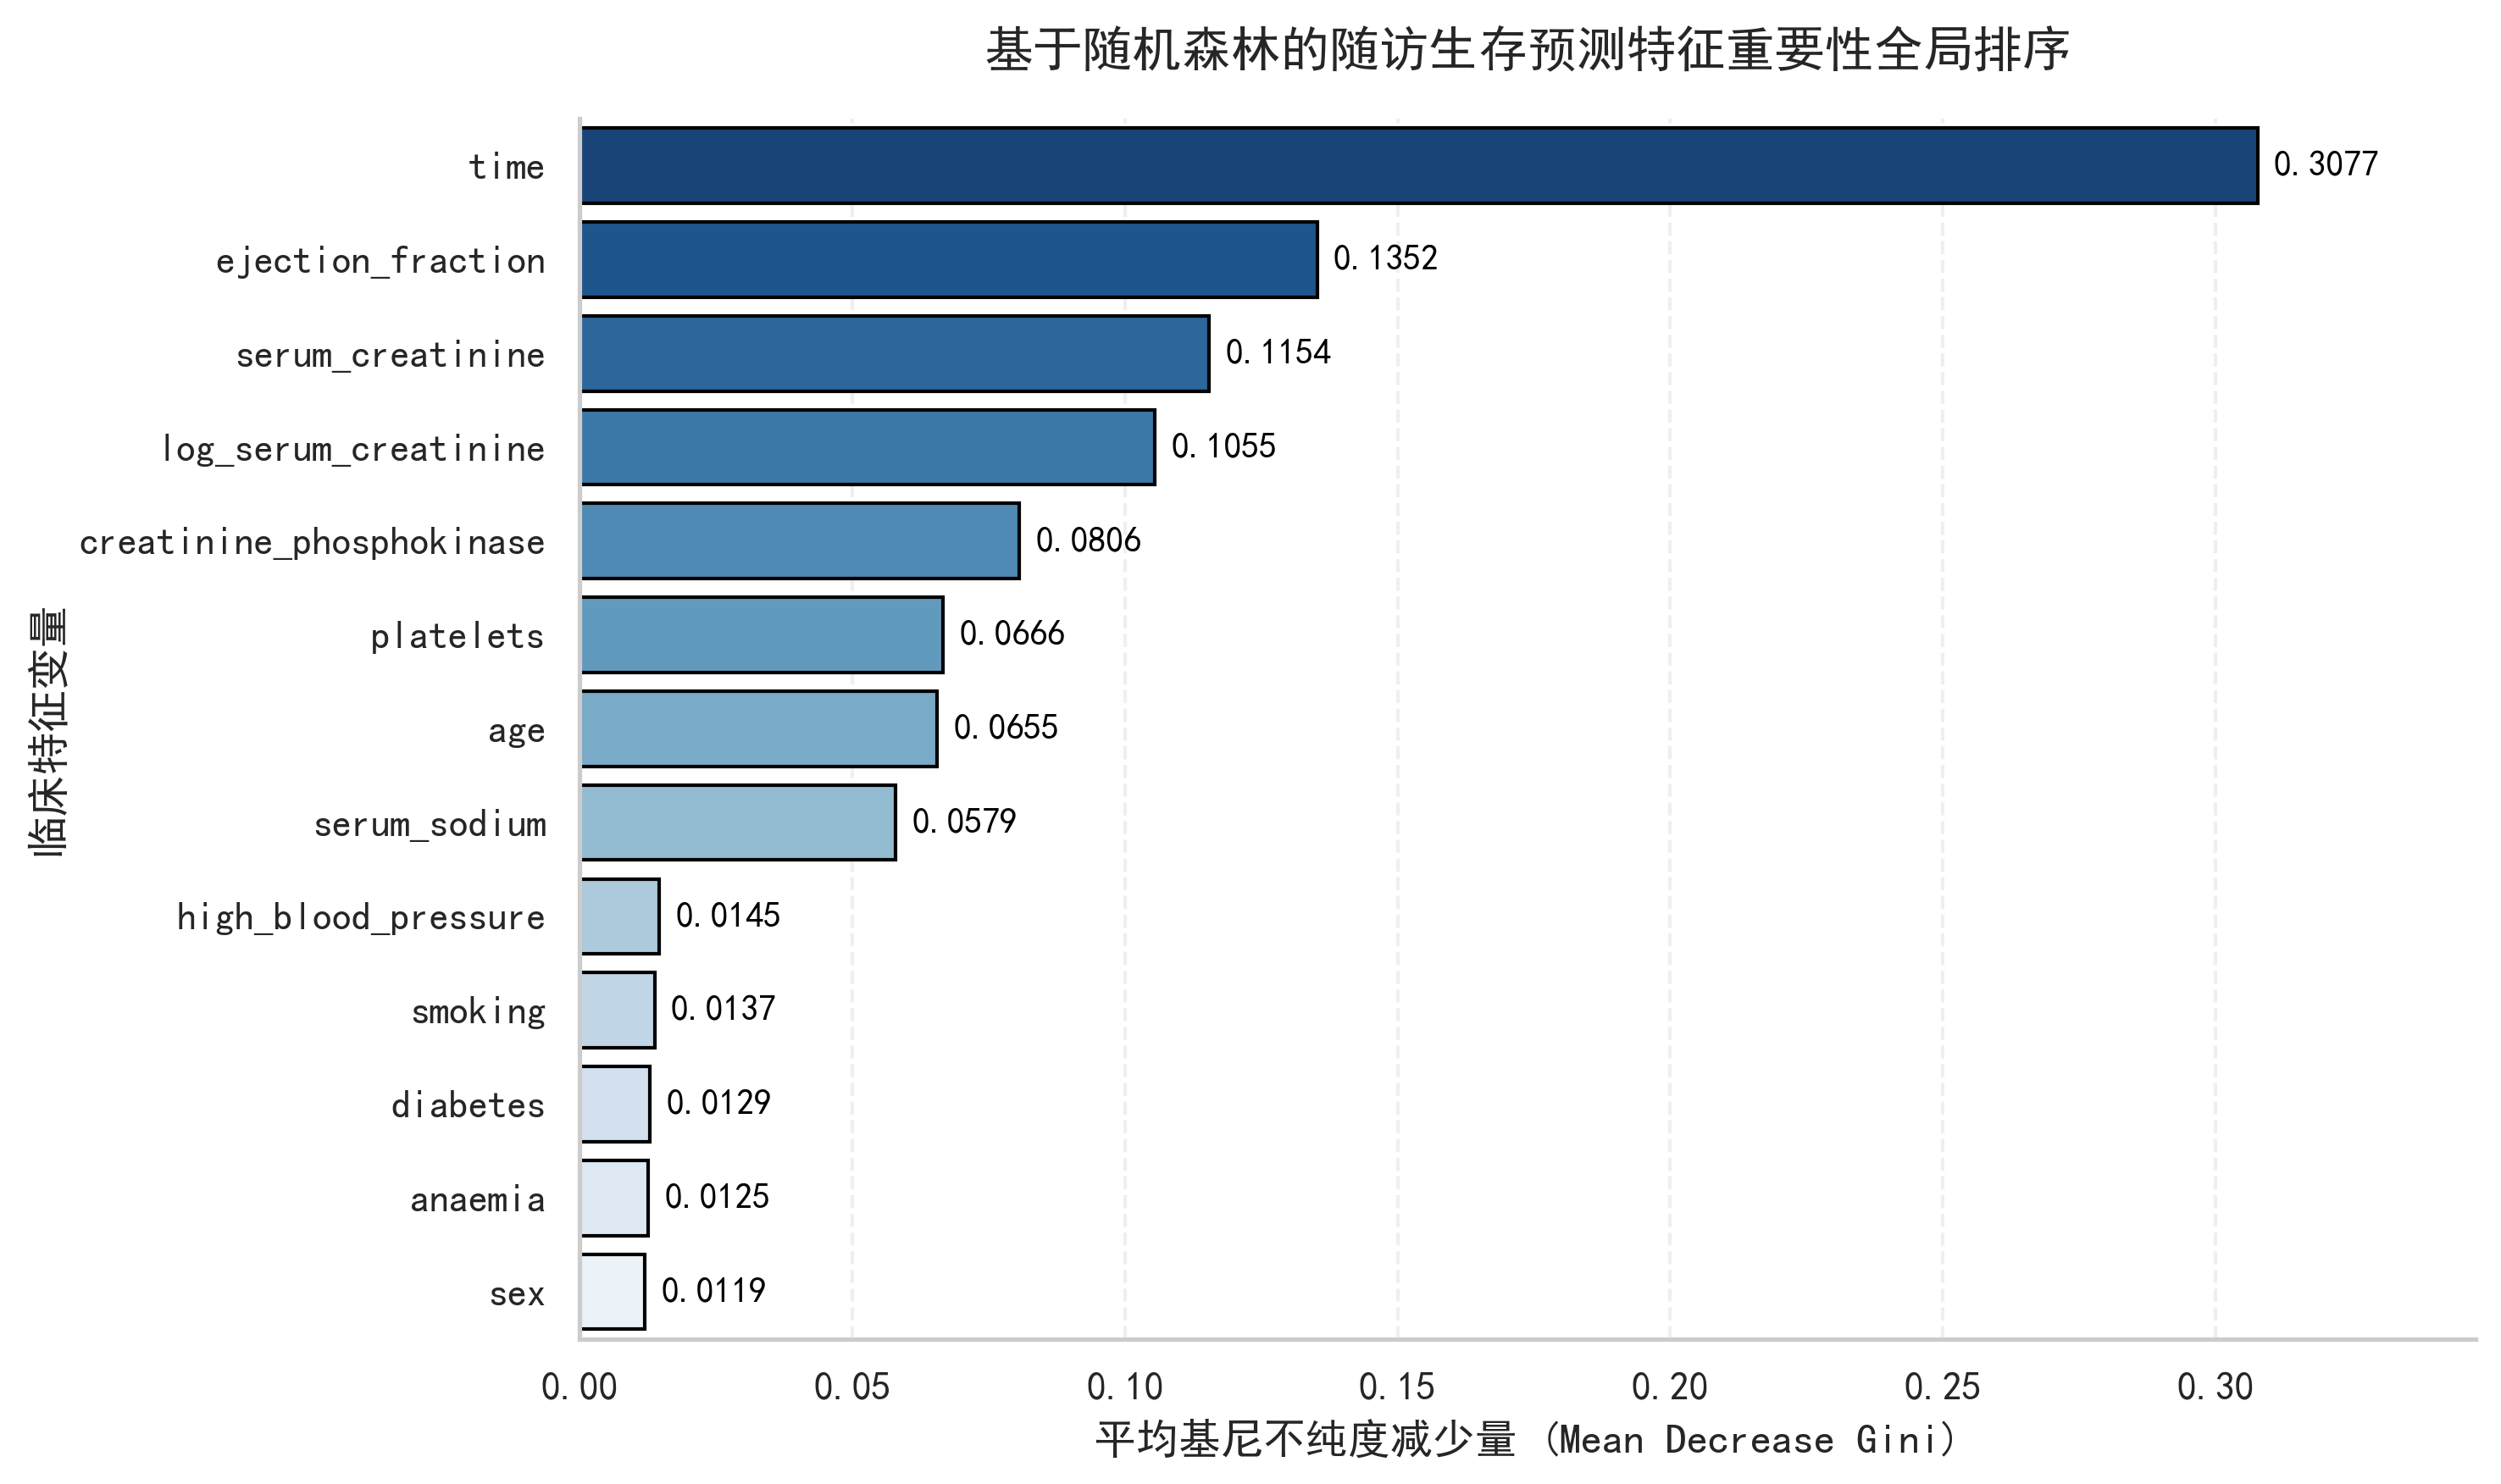
\includegraphics[width=\textwidth]{importance.png}
        \caption{基于随机森林的临床特征重要性排名}
        \label{fig:importance}
    \end{minipage}
\end{figure}

\begin{table}[H]
\centering
\caption{临床特征模型重要性权重与组间显著性检验表}
\label{tab:importance}
\small
\begin{tabular}{lrlcc}
\toprule
\textbf{临床特征变量} & \textbf{RF 权重} & \textbf{统计检验方法} & \textbf{\textit{p}-value} & \textbf{组间显著差异 (\textit{p}<0.05)} \\
\midrule
\texttt{随访时间} & $0.3077$ & 秩和检验 & $< 0.0001$ & 是 \\
\texttt{射血分数} & $0.1352$ & 秩和检验& $< 0.0001$ & 是 \\
\texttt{血清肌酐} & $0.1154$ & 秩和检验& $< 0.0001$ & 是\\
\texttt{对数转换后血清肌酐} & $0.1055$ & 秩和检验 & $< 0.0001$ & 是\\
\texttt{肌酸磷酸激酶} & $0.0806$ & 秩和检验 & $0.6841$ & 否 \\
\texttt{血小板计数} & $0.0666$ & 秩和检验 & $0.4253$ & 否 \\
\texttt{年龄} & $0.0655$ & 秩和检验& $0.0002$ & 是\\
\texttt{血清钠} & $0.0579$ & 秩和检验& $0.0003$ & 是\\
\texttt{高血压} & $0.0145$ & 卡方检验 & $0.2141$ & 否\\
\texttt{吸烟} & $0.0137$ & 卡方检验& $0.9318$ & 否 \\
\texttt{糖尿病} & $0.0129$ & 卡方检验& $1.0000$ & 否 \\
\texttt{贫血} & $0.0125$ & 卡方检验& $0.3073$ & 否 \\
\texttt{性别} & $0.0119$ & 卡方检验& $1.0000$ & 否 \\
\bottomrule
\end{tabular}
\end{table}

结果显示，随访时间、射血分数、血清肌酐三项指标重要性权重最高，分别为0.3077、0.1352、0.1154，且组间差异均达到极显著水平（$p<0.0001$）。随访时间越短、射血分数越低、血清肌酐越高，患者死亡风险越高，与心衰病理生理机制高度一致。年龄、血清钠亦表现显著差异，但预测贡献相对较低；而肌酸磷酸激酶、血小板计数、高血压、糖尿病、吸烟、贫血、性别均未显示统计学意义。上述三项核心因子在两组间分布差异显著，分层结果见图 \ref{fig:stratification}。

\begin{figure}[H]
    \centering
    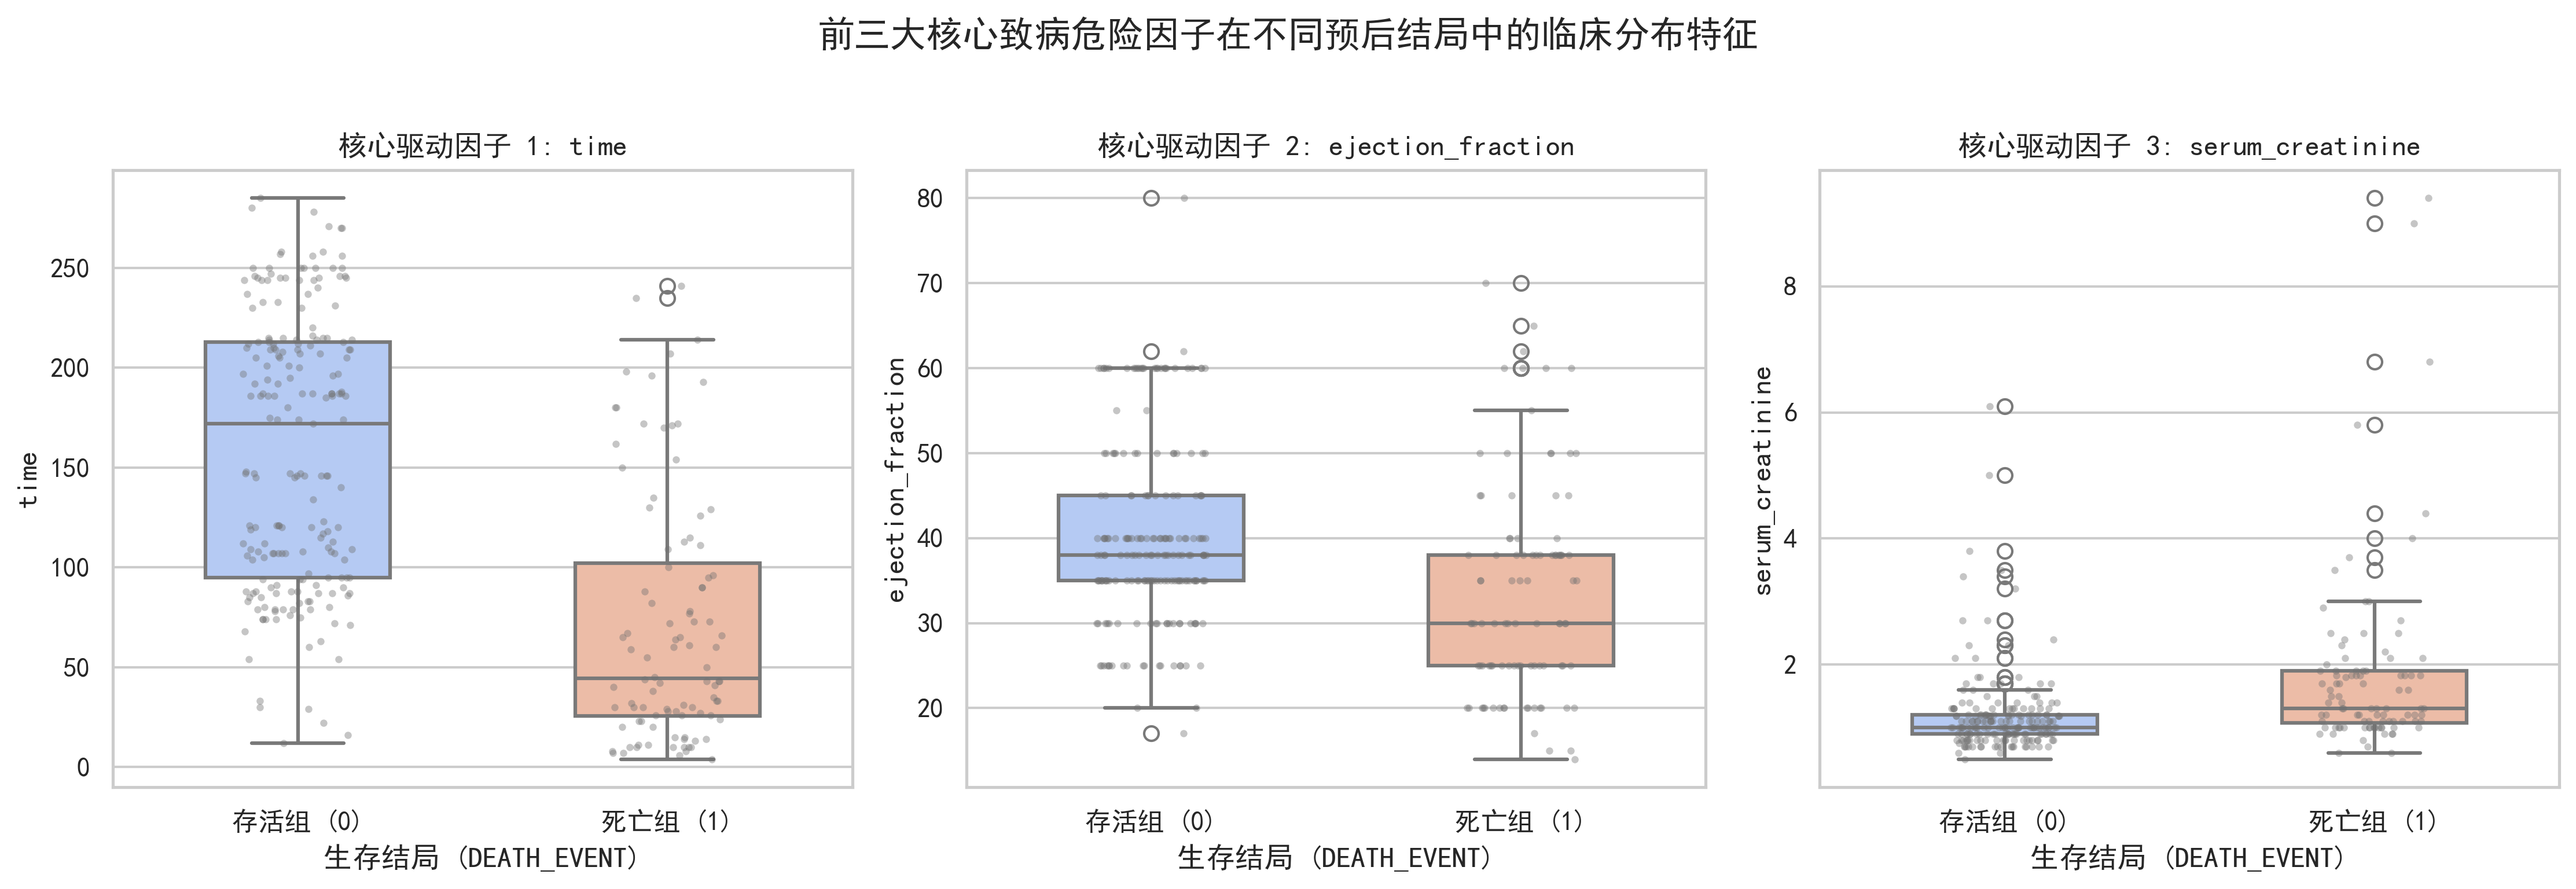
\includegraphics[width=0.75\textwidth]{前三大核心危险因子临床生存分层图.png}
    \caption{前三大核心危险因子在存活组与死亡组之间的箱线图分层差异}
    \label{fig:stratification}
\end{figure}

\subsection{独立测试集生存预测泛化表现}
心力衰竭数据存在类别不平衡（死亡比例32.11\%），单一准确率易高估模型性能，因此本研究采用多维度指标综合评估四种模型的泛化能力。独立测试集（$N=60$）结果如表 \ref{tab:performance}，ROC曲线与混淆矩阵见图 \ref{fig:roc_curve}。

\begin{table}[H]
\centering
\caption{多模型测试集生存预测泛化性能对比表}
\label{tab:performance}
\small
\begin{tabular}{lrrrrr}
\toprule
\textbf{评估模型} & \textbf{Accuracy} & \textbf{Precision} & \textbf{Recall} & \textbf{F1-Score} & \textbf{AUC} \\
\midrule
Logistic Regression & \num{81.67}\% & $0.7857$ & $0.5789$ & $0.6667$ & $0.85$ \\
Random Forest & \num{81.67}\% & $0.7500$ & $0.6316$ & $0.6857$ & $0.88$ \\
XGBoost & \num{81.67}\% & $0.7857$ & $0.5789$ & $0.6667$ & $0.84$ \\
MLP (Deep Learning) & \num{70.00}\% & $0.5294$ & $0.4737$ & $0.5000$ & $0.77$ \\
\bottomrule
\end{tabular}
\end{table}

\begin{figure}[H]
    \centering
    \begin{minipage}[t]{0.48\textwidth}
        \centering
        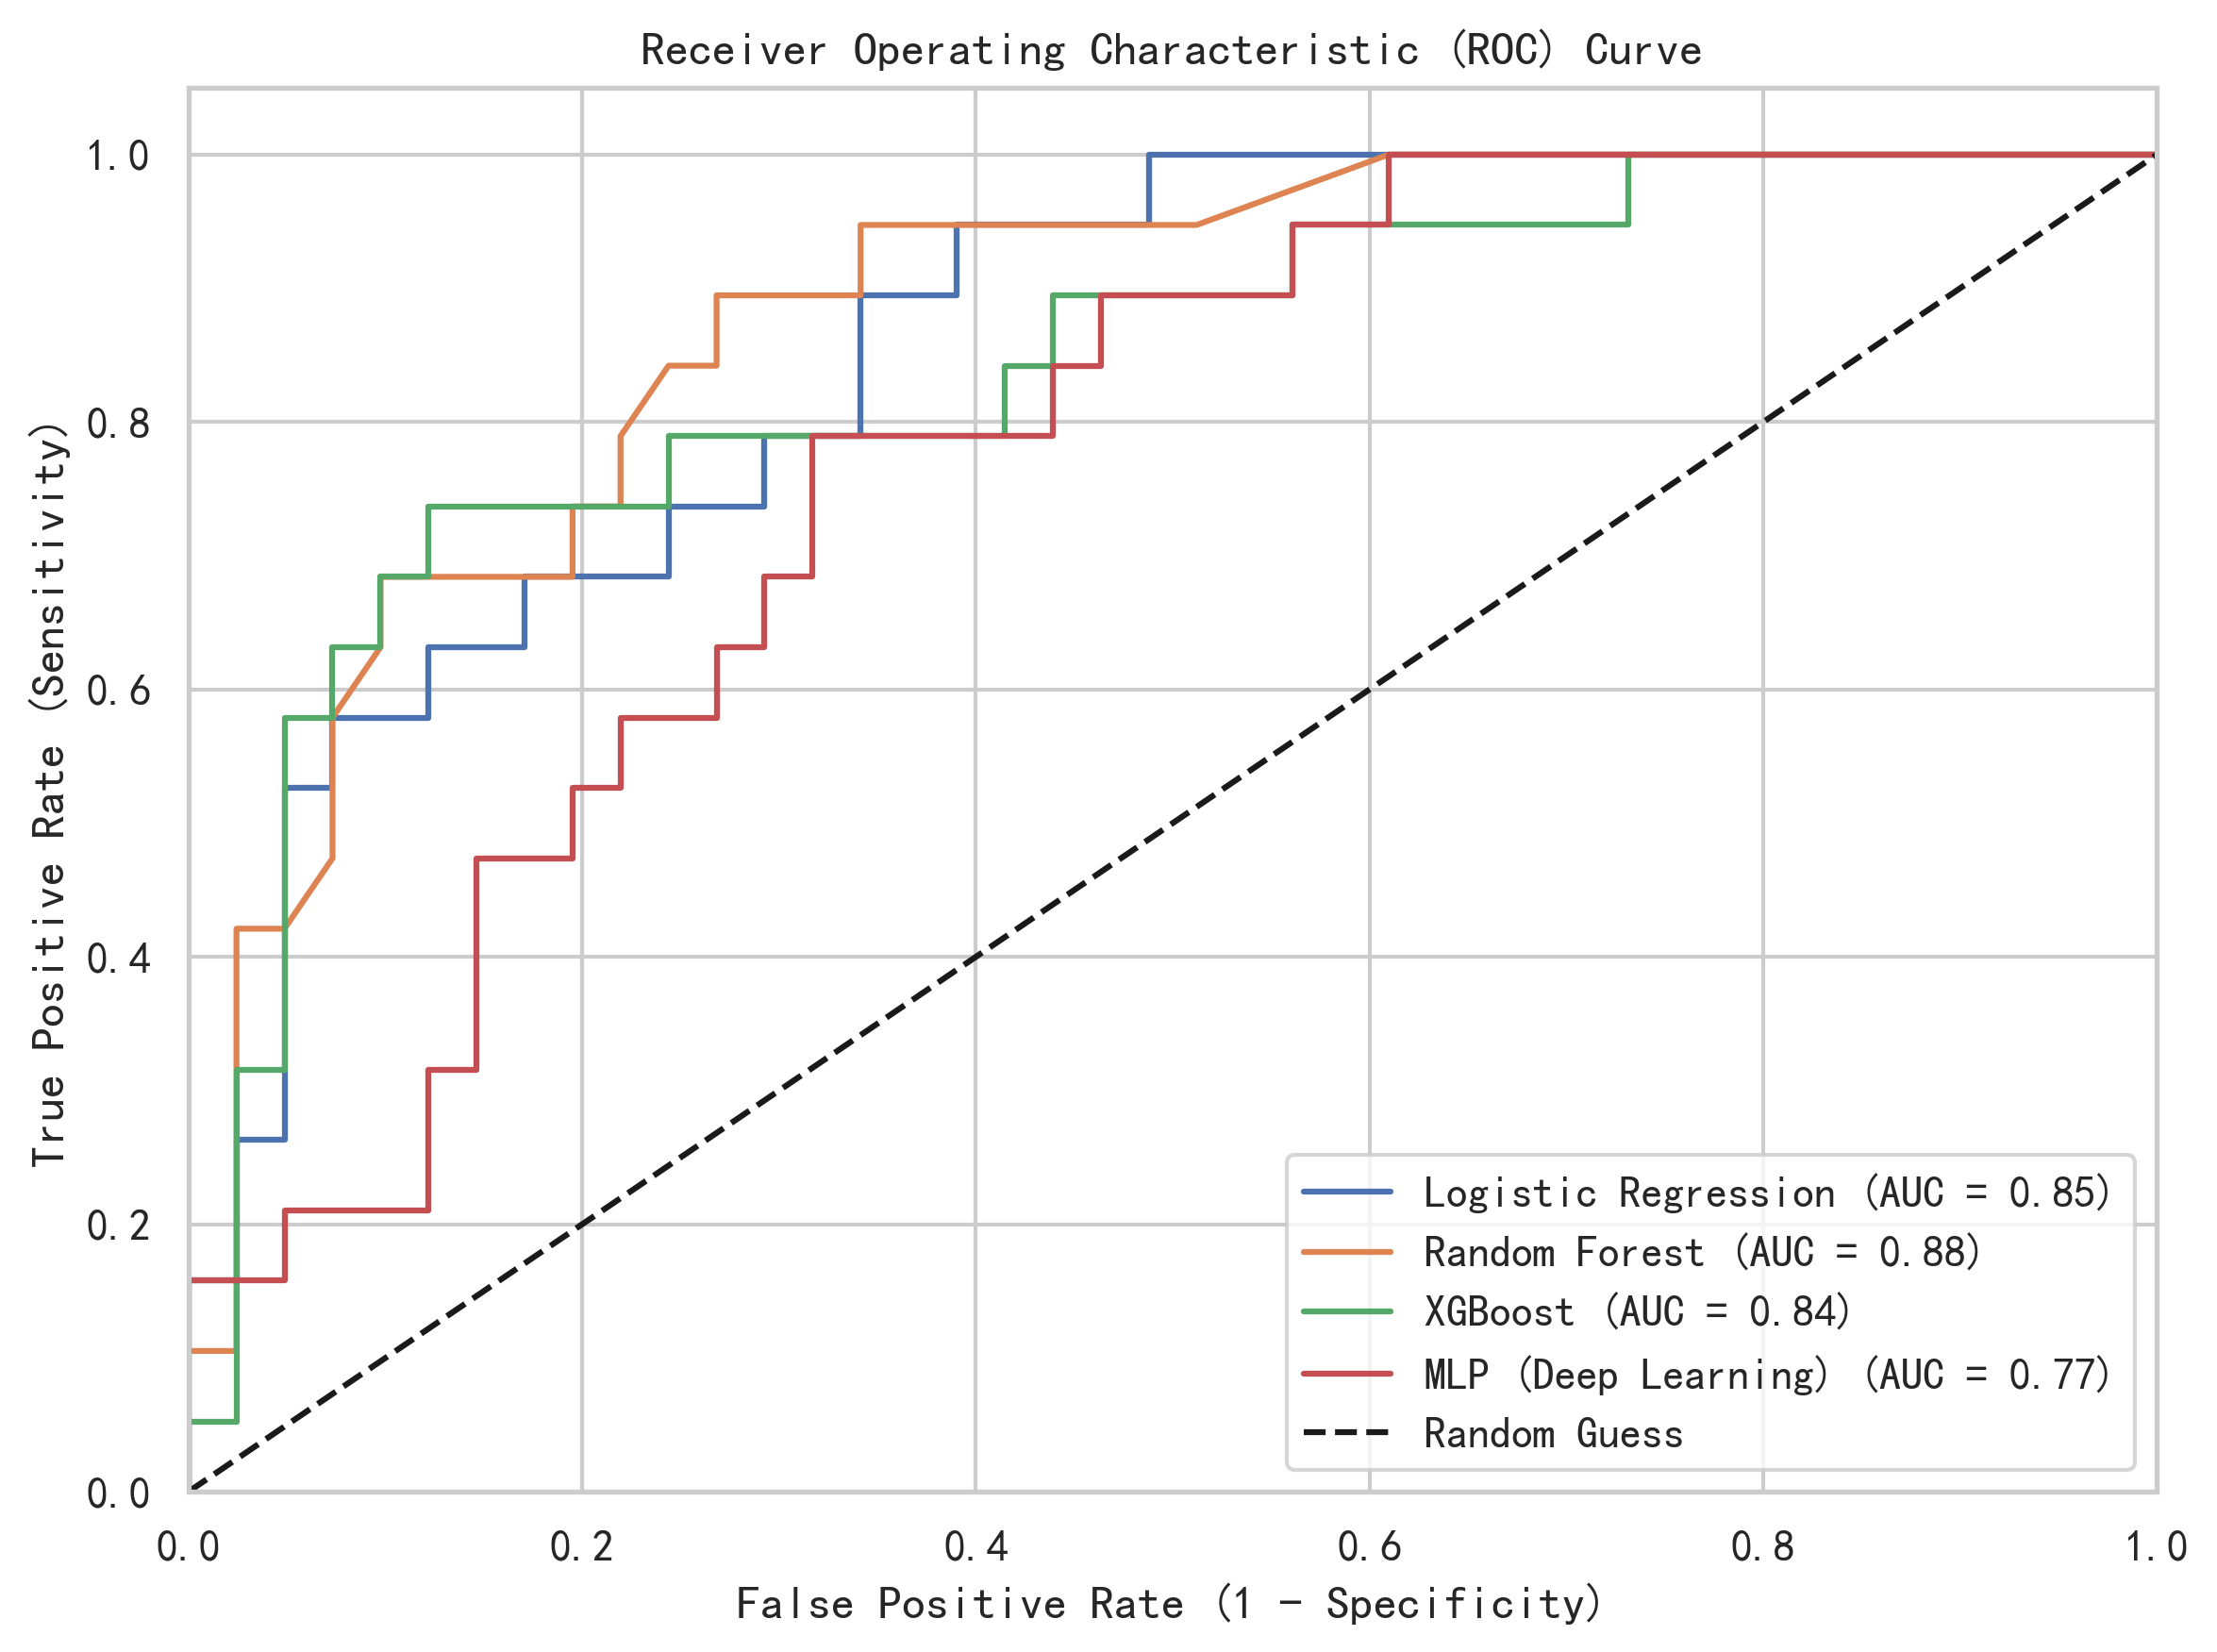
\includegraphics[width=\textwidth]{roc_curve.png}
        \caption{四种模型独立测试集受试者工作特征(ROC)曲线对比}
        \label{fig:roc_curve}
    \end{minipage}
    \hfill
    \begin{minipage}[t]{0.48\textwidth}
        \centering
        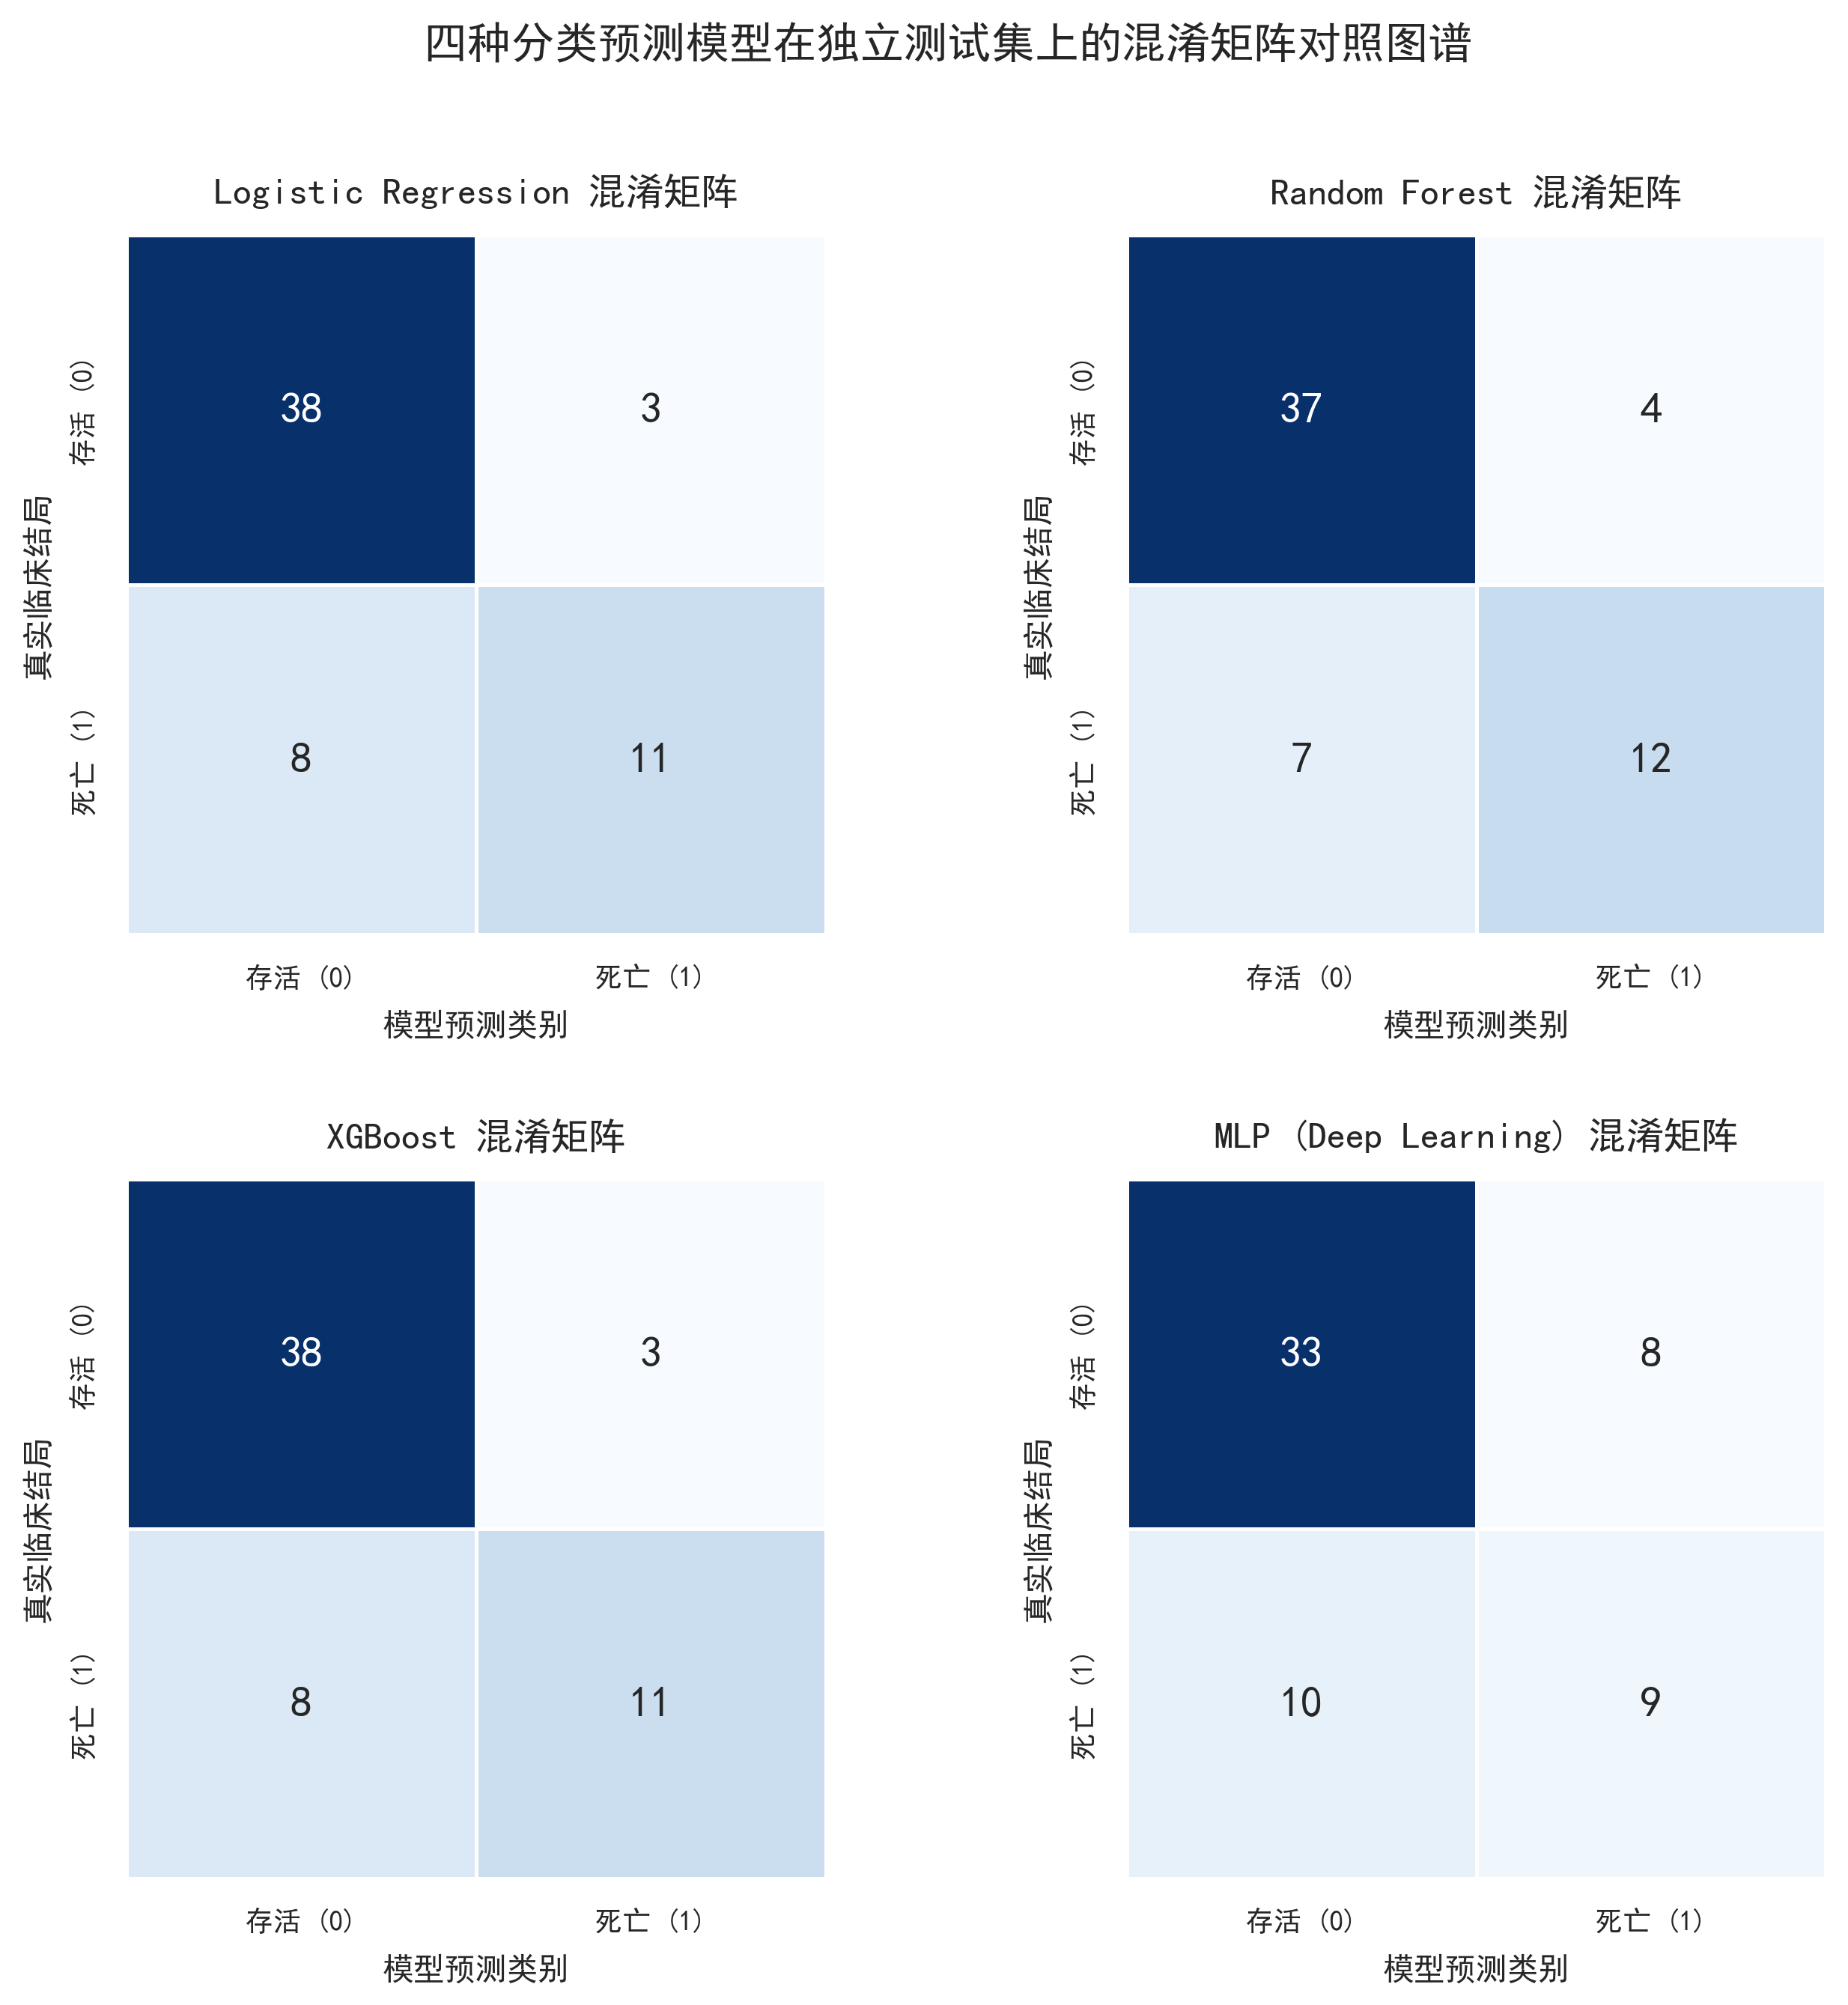
\includegraphics[width=\textwidth]{四模型混淆矩阵对比图.png}
        \caption{四种分类预测模型在独立测试集上的混淆矩阵对照图谱}
    \end{minipage}
\end{figure}

结果显示，传统机器学习与集成算法（LR、RF、XGBoost）在测试集准确率均为81.67\%，整体拟合能力相当。其中，随机森林综合性能最优，AUC=0.88、F1=0.6857、Recall=0.6316，表明其在高危患者识别中漏诊率最低，临床实用性最强。逻辑回归与XGBoost准确率相同，但召回率偏低，高危检出能力较弱。相比之下，MLP性能显著下滑，准确率仅70.00\%、AUC=0.77、精确率仅0.5294，假阳性比例高，易导致临床误判，提示深度学习在小样本表格数据中泛化能力不足。

\subsection{训练集与测试集过拟合风险的对比分析}
小样本医疗数据易引发过拟合，因此本研究通过AUC泛化衰减率量化模型稳定性，结果如表 \ref{tab:overfitting}。

\begin{table}[H]
\centering
\caption{四种模型训练集 vs 测试集过拟合风险分析表}
\label{tab:overfitting}
\small
\begin{tabular}{lrrrrr}
\toprule
\textbf{评估模型} & \textbf{Train Acc} & \textbf{Test Acc} & \textbf{Train AUC} & \textbf{Test AUC} & \textbf{AUC泛化衰减率 } \\
\midrule
Logistic Regression & \num{84.94}\% & \num{81.67}\% & $0.9095$ & $0.8549$ & $0.0545$ \\
Random Forest & \num{100.00}\% & \num{81.67}\% & $1.0000$ & $0.8761$ & $0.1239$ \\
XGBoost & \num{100.00}\% & \num{81.67}\% & $1.0000$ & $0.8395$ & $0.1605$ \\
MLP (Deep Learning) & \num{99.58}\% & \num{70.00}\% & $1.0000$ & $0.7677$ & $0.2323$ \\
\bottomrule
\end{tabular}
\end{table}

结果显示，逻辑回归泛化最稳，AUC衰减仅0.0545，拟合偏差最小。随机森林与XGBoost训练集完全拟合，但测试性能仍较高，过拟合可控。而MLP出现严重恶性过拟合，训练AUC=1.0、测试AUC=0.77，衰减高达0.2323，说明深度网络在小样本表格数据中易记忆噪声、泛化极差。综上，随机森林为最优模型，兼顾精度、稳定性与临床实用性。

\section{讨论}

\subsection{核心驱动因子的病理学映射}
本研究识别出的三大核心高危因子（随访时间、射血分数、血清肌酐）具有深厚的临床病理学印证。射血分数直接反映了左心室的收缩泵血效能，其数值在死亡组（$33.47 \pm 12.53\%$）中显著低于存活组（$40.27 \pm 10.86\%$），这与临床上“射血分数降低的心力衰竭（HFrEF）预后极差”的共识完全一致\cite{ponikowski2014heart}。

血清肌酐则是评估肾小球滤过率的核心实验室指标，心衰引发的体循环淤血和心排血量不足极易诱发心肾综合征（Cardiorenal Syndrome），导致死亡组的肌酐水平明显升高（$1.84$ vs $1.18\text{ mg/dL}$）\cite{ahmad2022survival}。这证明了本研究提取的机器学习特征权重并非单纯的数学拟合，而是具备高度可信的临床病理学生物学映射。

\subsection{小样本表格医疗数据下的模型选择策略}
表 \ref{tab:overfitting} 所记录的量化指标为临床数据建模中的算法选择给出了清晰的界定。全连接深度神经网络（MLP）由于其庞大的参数量，拥有极强的连续非线性函数逼近能力。然而，在医疗小样本表格任务（$N=299$）中，这种超高自由度反而成为其致命缺陷。

首先，表格数据特征之间不存在诸如图像的空间局部相关性先验，MLP 无法自适应地在极少的样本中提取泛化规则\cite{shickel2018deep}。由于缺少归纳偏置（Inductive Bias），MLP 在误差反向传播中深度记忆了 239 个训练样本的随机局部噪声（例如某个病人的高肌酸激酶与死亡结局的偶然偶发关联），从而将噪声当成了全局规律。

相反，集成算法如随机森林（RF）通过有放回的样本重采样（Bagging）和特征空间的随机子集投影，天生具备强大的方差控制机制\cite{breiman2001random}。即使其基分类器在训练集达到 $100\%$ 的过拟合极限，其通过多数投票机制构建的决策边界依然具备较高的容错空间与平滑度。这表明，在面对数百例级别的临床小样本 EHR 表格任务时，盲目追求深度学习网络往往无法获得红利，传统的树深度集成模型更具技术鲁棒性。

\subsection{研究局限性与未来改进方向}
尽管本研究构建的模型流线取得了优异的预后评估性能，但仍存在若干局限性：本研究样本量较小（$N=299$）且来自单一医疗中心，模型的外部泛化性能仍需在多中心独立队列中进行验证；目前仅采用了基线静态随访指标，未能整合患者在随访过程中的动态生命体征变化（如多节点动态心电图）；此外，目前将生存问题简化为了二分类任务，忽略了右删失数据的时间跨度不均性\cite{katzman2018deepsurv}。未来将致力于引入 Cox 比例风险模型与机器学习结合的生存网络（如 DeepSurv），直接对删失数据的生存函数进行精确建模。


\section{结论}
本研究构建了一套面向心力衰竭患者生存预后预测与临床风险因子识别的机器学习分析框架。基于公开心衰临床数据集的实验结果表明，结合对数变换预处理与集成树模型的分析流程具有稳定可靠的预测性能，具备作为临床决策支持工具的应用潜力，能够辅助临床医师开展患者风险分层与诊疗决策。随访时间、射血分数及血清肌酐被一致识别为影响心衰患者死亡结局的核心预测因子，具有显著统计学意义与明确的病理学解释价值。基于上述关键指标，本研究最优模型（随机森林）可精准识别高死亡风险的心衰患者。

本研究的局限性在于采用的数据集样本量相对有限且来自单一中心。引入更大规模、多中心、不同地域来源的临床队列，将有助于进一步验证模型的外部泛化能力，并更深入地揭示影响心衰患者预后的关键临床特征。

本研究系统对比了传统机器学习、集成算法与深度神经网络在医疗表格数据中的建模表现。多层感知机表现出严重的过拟合问题，而树基集成模型展现出优异的泛化鲁棒性。后续研究将进一步探索多种数据平衡策略、纳入动态时序临床信息，并融合Cox比例风险模型等生存分析方法，以进一步提升心衰患者生存预后预测的精准度与临床实用性。

\newpage
\begin{thebibliography}{10}

\bibitem{chicco2020machine}
Chicco D, Jurman G.
\newblock Machine learning can predict survival of patients with heart failure from serum creatinine and ejection fraction alone.
\newblock {\em BMC Medical Informatics and Decision Making}, 2020, 20(1): 16.

\bibitem{newaz2021survival}
Newaz A, Ahmed N, Haq FS.
\newblock Survival prediction of heart failure patients using machine learning techniques.
\newblock {\em Informatics in Medicine Unlocked}, 2021, 26: 100772.

\bibitem{ahmad2022survival}
Ahmad T, Munir A, Bhatti SH, et al.
\newblock Survival analysis of heart failure patients: A clinical record-based study utilizing machine learning classification algorithms.
\newblock {\em PLOS ONE}, 2022, 17(4): e0265191.

\bibitem{ponikowski2014heart}
Ponikowski P, Anker SD, AlHabib KF, et al.
\newblock Heart failure: preventing disease and death worldwide.
\newblock {\em ESC Heart Failure}, 2014, 1(1): 4--25.

\bibitem{katzman2018deepsurv}
Katzman JL, Shaham U, Cloninger A, et al.
\newblock DeepSurv: personalized treatment recommender system based on a Cox proportional hazards deep neural network.
\newblock {\em BMC Medical Research Methodology}, 2018, 18(1): 24.

\bibitem{breiman2001random}
Breiman L.
\newblock Random Forests.
\newblock {\em Machine Learning}, 2001, 45(1): 5--32.

\bibitem{chen2016xgboost}
Chen T, Guestrin C.
\newblock XGBoost: A scalable tree boosting system.
\newblock In {\em Proceedings of the 22nd ACM SIGKDD International Conference on Knowledge Discovery and Data Mining}, 2016: 785--794.

\bibitem{shickel2018deep}
Shickel B, Tighe PJ, Bihorac A, et al.
\newblock Deep EHR: A survey on deep learning techniques for electronic health record analytics.
\newblock {\em IEEE Journal of Biomedical and Health Informatics}, 2018, 22(2): 589--603.

\bibitem{lundberg2017unified}
Lundberg SM, Lee SI.
\newblock A unified approach to interpreting model predictions.
\newblock {\em Advances in Neural Information Processing Systems (NeurIPS)}, 2017, 30: 4765--4774.

\bibitem{benjamin2019heart}
Benjamin EJ, Muntner P, Alonso A, et al.
\newblock Heart disease and stroke statistics—2019 update: a report from the American Heart Association.
\newblock {\em Circulation}, 2019, 139(10): e56--e528.

\bibitem{tabular2022}
Grinsztajn L, Oyallon E, Varoquaux G.
\newblock Why do tree-based models still outperform deep learning on tabular data?.
\newblock {\em Advances in Neural Information Processing Systems (NeurIPS)}, 2022, 35: 507--520.

\end{thebibliography}

\end{document}
